\documentclass[hidelinks,12pt]{article}
\usepackage[left=0.25cm,top=1cm,right=0.25cm,bottom=1cm]{geometry}
%\usepackage[landscape]{geometry}
\textwidth = 20cm
\hoffset = -1cm
\usepackage[utf8]{inputenc}
\usepackage[spanish,es-tabla]{babel}
\usepackage[autostyle,spanish=mexican]{csquotes}
\usepackage[tbtags]{amsmath}
\usepackage{nccmath}
\usepackage{amsthm}
\usepackage{amssymb}
\usepackage{mathrsfs}
\usepackage{graphicx}
\usepackage{subfig}
\usepackage{standalone}
\usepackage[outdir=./Imagenes/]{epstopdf}
\usepackage{siunitx}
\usepackage{physics}
\usepackage{color}
\usepackage{float}
\usepackage{hyperref}
\usepackage{multicol}
%\usepackage{milista}
\usepackage{anyfontsize}
\usepackage{anysize}
%\usepackage{enumerate}
\usepackage[shortlabels]{enumitem}
\usepackage{capt-of}
\usepackage{bm}
\usepackage{relsize}
\usepackage{placeins}
\usepackage{empheq}
\usepackage{cancel}
\usepackage{wrapfig}
\usepackage[flushleft]{threeparttable}
\usepackage{makecell}
\usepackage{fancyhdr}
\usepackage{tikz}
\usepackage{bigints}
\usepackage{scalerel}
\usepackage{pgfplots}
\usepackage{pdflscape}
\pgfplotsset{compat=1.16}
\spanishdecimal{.}
\renewcommand{\baselinestretch}{1.5} 
\renewcommand\labelenumii{\theenumi.{\arabic{enumii}})}
\newcommand{\ptilde}[1]{\ensuremath{{#1}^{\prime}}}
\newcommand{\stilde}[1]{\ensuremath{{#1}^{\prime \prime}}}
\newcommand{\ttilde}[1]{\ensuremath{{#1}^{\prime \prime \prime}}}
\newcommand{\ntilde}[2]{\ensuremath{{#1}^{(#2)}}}

\newtheorem{defi}{{\it Definición}}[section]
\newtheorem{teo}{{\it Teorema}}[section]
\newtheorem{ejemplo}{{\it Ejemplo}}[section]
\newtheorem{propiedad}{{\it Propiedad}}[section]
\newtheorem{lema}{{\it Lema}}[section]
\newtheorem{cor}{Corolario}
\newtheorem{ejer}{Ejercicio}[section]

\newlist{milista}{enumerate}{2}
\setlist[milista,1]{label=\arabic*)}
\setlist[milista,2]{label=\arabic{milistai}.\arabic*)}
\newlength{\depthofsumsign}
\setlength{\depthofsumsign}{\depthof{$\sum$}}
\newcommand{\nsum}[1][1.4]{% only for \displaystyle
    \mathop{%
        \raisebox
            {-#1\depthofsumsign+1\depthofsumsign}
            {\scalebox
                {#1}
                {$\displaystyle\sum$}%
            }
    }
}
\def\scaleint#1{\vcenter{\hbox{\scaleto[3ex]{\displaystyle\int}{#1}}}}
\def\bs{\mkern-12mu}


\usepackage{apacite}
\title{Hint para el sistema coordenado toroidal \\[0.3em]  \large{Matemáticas Avanzadas de la Física}\vspace{-3ex}}
\author{M. en C. Gustavo Contreras Mayén}
\date{ }
\begin{document}
\vspace{-4cm}
\maketitle
\fontsize{14}{14}\selectfont

\section{Coord. toroidales \texorpdfstring{$(\eta, \theta, \psi)$}{(e, t, p)}.}

\subsection{Dominio de las coordenadas.}

\begin{align*}
0 &\leq \eta < +\infty \\
-\pi &< \theta \leq +\pi \\
0 &\leq \psi < 2 \, \pi
\end{align*}

\subsection{Reglas de transformación.}

\begin{align*}
x &= \dfrac{a \, \sinh \eta \, \cos \psi}{\cosh \eta - \cos \theta} \\[0.5em]
y &= \dfrac{a \, \sinh \eta \, \sin \psi}{\cosh \eta - \cos \theta} \\[0.5em]
z &= \dfrac{a \, \sin \theta}{\cosh \eta - \cos \theta}
\end{align*}

\subsection{Factores de escala.}

Deben de obtener de manera explícita estos factores:

\begin{align*}
(h_{1})^{2} = (h_{2})^{2} &= \dfrac{a^{2}}{(\cosh \eta - \cos \theta)^{2}} \\[0.5em]
(h_{3})^{2} &= \dfrac{a^{2} \, \sinh^{2} \eta}{(\cosh \eta - \cos \theta)^{2}}
\end{align*}

\subsection{Superficies coordenadas.}

De la gráfica que se incluye en las notas de trabajo, tenemos que:

\begin{figure}[H]
    \centering
    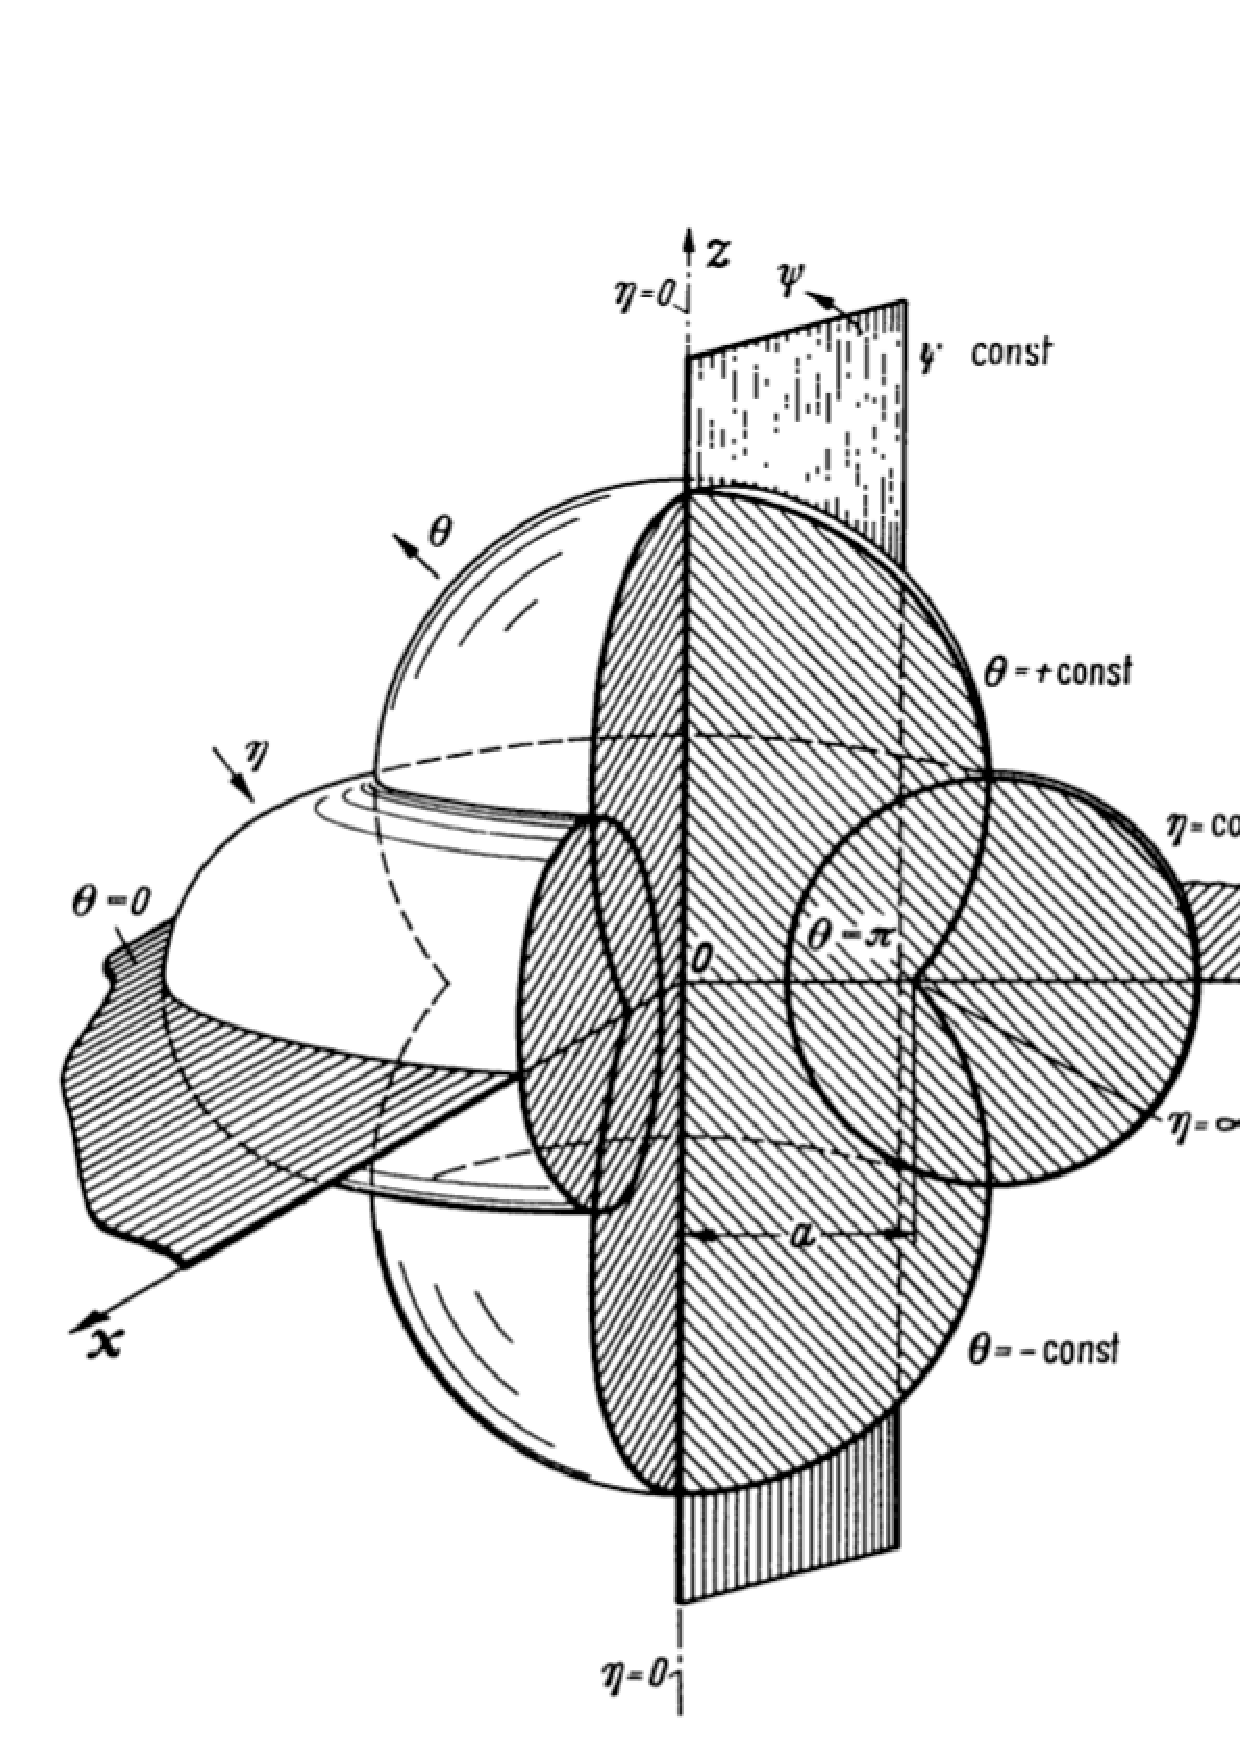
\includegraphics[scale=0.4]{Imagenes/Sistema_Toroidal.pdf}
    \caption{Sistema coordenado toroidal.}
\end{figure}

Como apoyo, deben de manejar las variables de tal manera para obtener:

\begin{align}
x^{2} + y^{2} + z^{2} + a^{2} &= 2 \, a \, (x^{2} + y^{2})^{\frac{1}{3}} \, \coth \eta \label{eq:superficie_01} \\[0.5em]
x^{2} + y^{2} + (z - a \cot \theta)^{2} &= \dfrac{a^{2}}{\sin^{2} \theta} \label{eq:superficie_02} \\[0.5em]
\tan \psi &= \dfrac{y}{x} \label{eq:superficie_03}
\end{align}

donde las superficies coordenadas son:
\begin{enumerate}
\item Con $\eta$ = constante en la ec. (\ref{eq:superficie_01}) se obtienen toroides.
\item Con $\theta$ = constante en la ec. (\ref{eq:superficie_02}) se obtienen cuencos esféricos.
\item Con $\psi$ = constante en la ec. (\ref{eq:superficie_03}) se obtienen medios planos.
\end{enumerate}

Toma en cuenta que la referencia te está diciendo la superficie obtenida, por lo que en tu manejo debes de manipular las correspondientes variables y llegar a esas ecuaciones, te puedes apoyar también indicando la ecuación general para cada una de las superficies mencionadas.

\end{document}